\chapter{Software Design, Implementation and Testing}

% This could be one chapter or a few chapters. It should define and discuss the software that is developed to support the research that is being conducted. For example, if your research involves running experiments, 
% 
% What software are you creating to support that work?

\section{Requirements}
There are two main components to the software being developed for this project. The first is the manipulation of the data into a database, and the second is a web front end for the data to be accessed via. 

\subsection{Database}
The database has to store the following information for each hit from the alignment with \textit{C. albicans}:

\begin{itemize}
  \item ID of the hit that was found when the species coding sequences have been aligned with \textit{C. albicans}.
  \item Species it came from.
  \item The gene name and ID from Candida Genome Database.
  \item UniProt ID.
  \item Contig of raw DNA.
  \item Coding sequence of nucleotides.
  \item Protein sequence that the coding sequence codes for.
  \item Annotations from NCBI nr database to provide a description of the proteins.
  \item A list of Gene Ontology\cite{geneontology} ID's for the protein.
  \item If it can be found, the positions of the start and end of the coding sequence in the raw contig. 
\end{itemize}

From these requirements it is clear there are a few pieces of data that need to be extracted from the data that has been collated. For each alignment with \textit{C. albicans} the protein sequence and GO annotations need to found, the coding sequence that was used in the alignment and the contig that it came from. In addition to this the metadata about the genes such as the name and ID's need to be read from the mapping file that was created earlier. 

The final bit of data that needs to be added is the position of the coding sequence in the contig. An algorithm will have to be developed to detect this.

\subsection{Website}
The website will only have a few requirements: 

\begin{itemize}
  \item Display each record in the database in an easy to read manner. 
  \item Highlight coding sequence in contig if possible.
  \item Copy coding sequence and +/- a user defined number of bases to the clipboard.
  \item Search the database for a gene, but name, description, ID, or even by nucleotide sequence. 
\end{itemize}

\section{Build Process}
  One of the first things that was setup for this project was the build process. This doesn't take long to setup but provides a huge benefit for the rest of the project. It helps to reduce errors and speed up the process of deployment and testing.

  \subsection{Development Environment}
    This project will be developed on an Arch Linux system, as it will only ever be ran on a Linux host this isn't an issue, as the production environment will match the development one. 

    All of the code and LaTeX will be written with the editor Vim, which has been configured to have many optimisations to this workflow. The full Vim configuration that was used can be found here\cite{vimrc}.

  \subsection{Code Style}
  For this project the Clock Limited code standard\cite{clockstandard} will be followed. This has a few key variations to typical Javascript. 

  \begin{itemize}
    \item Semicolons are not required in JS, so they are not used to denote EOL.
    \item Strings are encapsulated with single quotes, not double. 
    \item Comma first\cite{commafirst} listing of variables, objects and arrays.
    \item No commenting, to avoid confusion, encourage descriptive naming and reduce file length.
  \end{itemize}

  These rules ensure that the code written is clean and easy to read.

  \subsection{Version Control}
    This project is being entirely tracked with Git version control. This allows the developer to have all of the work backed up, with an easily accessible history. It also allows for branching of the project to test out experimental features or bug fixes. The project is remotely hosted on Github\cite{github} for remote backup and access via multiple hosts. Github also is widely supported for third party integrations, something that will be utilised quite extensively. 

    When pushing code to Github, a module called Husky\cite{husky} will run the test suite on the developers local machine. If the tests fail, the code will not be pushed.

  \subsection{Test suite}
    The test suite is set up to first clean the project of old builds and coverage reports, then run ESlint\cite{eslint}. This will scan the entire codebase for files that do not adhere to the code style defined in the Clock configuration. This means that any badly formatted code will cause an error and prevent the code from being pushed until the developer fixes the issues. 

    After the linting check, the test suite will use Mocha\cite{mocha} to run all of the JavaScript test files that are in the project. If any of the assertions made in the test files fail, the project will not be pushed. 

    Once the test's have been ran Istanbul\cite{istanbul} will provide a coverage report, that will show to the user the percentage of tested code that has been covered by the assertions. After this the code can finally be pushed to Github. 
    
  \subsection{Continuous Integration}
    Once the code has been pushed to Github, a hook on Github will trigger Travis CI\cite{travis} to clone down the latest version of the code to it's servers and run the test suite again on it's own server. This is very useful as occasionally developers can bypass Husky to push code, or have something setup in their system that isn't defined in the application that causes test to pass on their system but not when the application is built from scratch. 

    Once those tests are successful, it will send the coverage report generated by Istanbul to another third party service called Codecov\cite{codecov}. This tracks the test coverage over time and provides interactive charts highlighting areas that need more test coverage. 

\begin{figure}[H]
\begin{center}
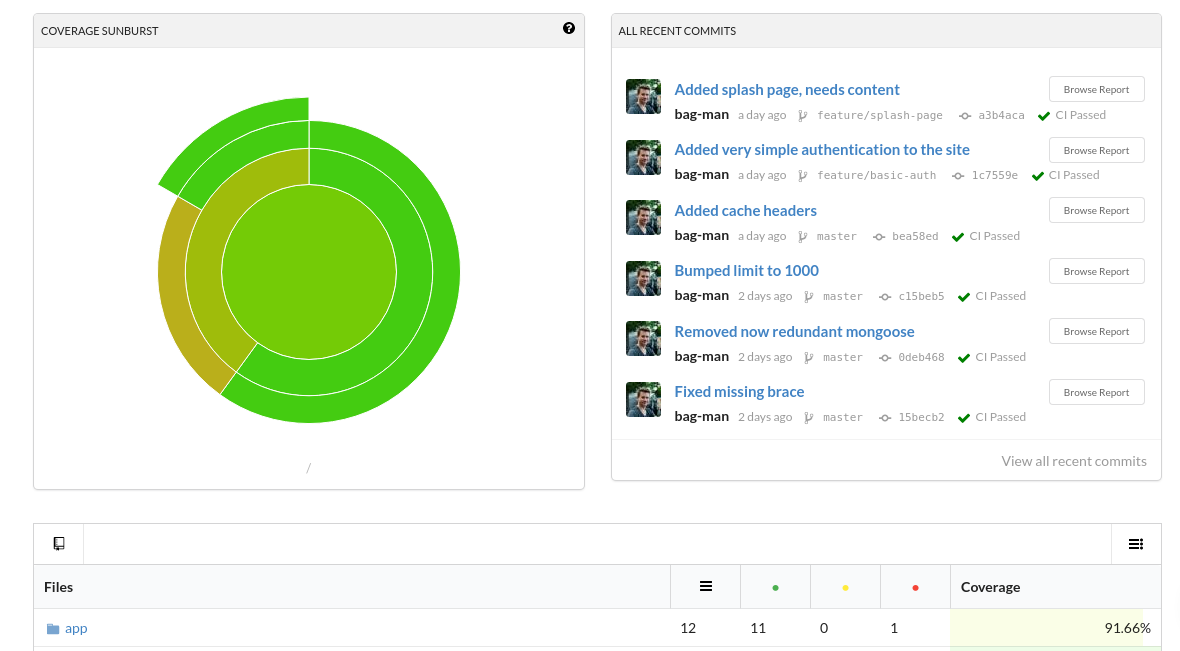
\includegraphics[scale=0.4]{codecov}
\caption{Codecov interactive coverage report}
\end{center}
\end{figure}



  \subsection{Deployment}
  If the tests pass on Travis CI, a Github hook will then activate the deployment. The project is setup to use Heroku\cite{heroku}, and to build on successful CI results. This means that when code is pushed to the master branch, it will automatically be deployed to their service. This is excellent for development as it allows changes made to the system to be almost immediately reflected on the live website. The only drawback of Heroku is that this project is using their free offerings which only allow 500MB's of database storage, which means that anything larger than that will be truncated. This isn't an issue for development, however it will mean that when the project is to go live, funding would need to be found to pay for more data storage, or alternatively the project can be hosted elsewhere, most likely within the University network.

  The benefits of this build process are clear, firstly code is automatically deployed, which saves the developers a lot of time, as well as encouraging regular client feedback. However the main advantage is that before the deployment the code will have had the test suite ran on it twice, once on the developers local machine and then again on a brand new build on the CI service. This means that any mistakes are caught before they are put into production and the developer is notified of these issues so they can't be avoided. 


\section{Design}
% You should concentrate on the more important aspects of the design. It is essential that an overview is presented before going into detail. As well as describing the design adopted it must also explain what other designs were considered and why they were rejected.
% 
% What design will be used?
% 
% What implementation issues are there and what testing is used? 
% 
% Even though a research project is investigating specific research questions, it is still necessary for you to discuss the software that you develop. Research has a habit of generating bits of software that can exist for several years and need future modification. Therefore you need to be able to discuss the technical issues as well as the research approach. 

The first stage in designing this system was to decide upon what database technology would be used for the data store. As discussed in the analysis a NoSQL database called MongoDB has been chosen to store the data. This choice was also influenced by the choice of server side language, which for this project will be NodeJS. 

NodeJS was chosen because:

\begin{itemize}
  \item Client and server side languages are the same.
  \item Integrates well with MongoDB as it uses BSON which works with native JSON.
  \item Provides easy package management via npm.
  \item ES6 syntax is very nice.
  \item I have a lot of experience with it and learning a new language is outside of the scope of the project.
\end{itemize}

As outlined in Ioannis K. Chaniotis et al's paper, `Our study concludes that Node.js offers client-server development integration, aiding code reusability in web applications, and is the perfect tool for developing fast, scalable network applications.'\cite{node-perf}

The website for this interface will be built off of nodestack\cite{nodestack}, a set of boilerplate code that uses several technologies including:


\begin{itemize}
  \item Node JS / ES6

    "Node.js is a JavaScript runtime built on Chrome's V8 JavaScript engine. Node.js uses an event-driven, non-blocking I/O model that makes it lightweight and efficient. Node.js' package ecosystem, npm, is the largest ecosystem of open source libraries in the world."\cite{node-org}
    Since Node >4.0 it has supported the ES6 standard, which provides a lot of syntactic sugar, and makes the formatting of the code a lot easier to read and write. 
  \item Webpack
    
    Webpack is a module bundler that allows for easy packaging of client side javascript. It allows the client side javascript to be written in ES6, then when built it will transpile the ES6 code into more widely supported ES2015 code, minify it for efficient, and package it into one single file. This means that the code can be written in a nicely organised manner across multiple files in ES6, and then reduced to one small file for actual usage. 

  \item Mongoose

    Mongoose is an Object Data Manager, it allows developers to define schema's and validation for their data objects as well as extensible models for those objects. This makes interactions with MongoDB a lot simpler, as well as easy enforcement of validation rules.

  \item Pug

    Pug is an HTML templating language that allows developers to write HTML with dynamic variables from the server side, and include some logic elements. The main benefit is that it has a much cleaner syntax than HTML so it is a lot easier to read and write. 

  \item Stylus

    Stylus is an expressive CSS language that, like Pug and ES6, improves the syntax of CSS by minimising unnecessary elements. It has many other advantages over CSS, although for this project they aren't likely to be utilised as the front end design work of this project will be minimal. 

  \item Bootstrap

    Bootstrap is a CSS and JS framework that is aimed at making responsive websites easier to write. With the addition of bootstrap to the project adapting the front end to work on mobile will be minimal. It also adds useful features for laying out the page and some attractive default CSS. 
\end{itemize}


Using this boilerplate will save a huge amount of time in development as the basic framework of the web application is already laid out, so the development time can be focussed on developing software to meet the functional requirements rather than investing time in setting up a good web framework. 

For more detail on how the boiler plate works, you can read the guide here: \url{http://blog.owen.cymru/nodejs-es6-boiler-plate/}

\subsection{Database Import}
To import the genenomic data into the database from the fasta file format, a script will be written that will use a npm module called fasta2json\cite{fasta2json} to read the fasta files into JSON format. 

From there it will use the blast results generated by the diamond script to look up the cotnig, coding sequence, and amino acid sequence (protein) for each of the blast results. 

It will also compare the hit ID with the mappings file that was produced to get the ID's for the equivalent Uniprot and Candida Genome Database hits, if they are available. 

That data will then be inserted into MongoDB, and an index built on the searchable fields. This index will allow for a very fast and efficient search for the key fields that will be searched for in the database, description, gene name and ID's.

\begin{lstlisting}[caption=The database schema that will represent the hit object]
  { id: Schema.ObjectId
  , hitid: String
  , species: String
  , name: String
  , cgdid: String
  , uniprot: String
  , contig: 
    { head: String
    , seq: String 
    }
  , codingseq: 
    { head: String
    , seq: String 
    }
  , protein: 
    { head: String
    , seq: String
    , goids: [String]
    , desc: String 
    }
  , codingRange: 
    { start: Number
    , end: Number
    , fail: Boolean 
    }
  }
\end{lstlisting}

    

% The design should describe what you expected to do, and might also explain areas that you had to revise after some investigation.

% Typically, for an object-oriented design, the discussion will focus on the choice of objects and classes and the allocation of methods to classes. The use made of reusable components should be described and their source referenced. Particularly important decisions concerning data structures usually affect the architecture of a system and so should be described here.

% How much material you include on detailed design and implementation will depend very much on the nature of the project. It should not be padded out. Think about the significant aspects of your system. For example, describe the design of the user interface if it is a critical aspect of your system, or provide detail about methods and data structures that are not trivial. Do not spend time on long lists of trivial items and repetitive descriptions. If in doubt about what is appropriate, speak to your supervisor.
 
% You should also identify any support tools that you used. You should discuss your choice of implementation tools - programming language, compilers, database management system, program development environment, etc.

% Some example sub-sections may be as follows, but the specific sections are for you to define. 

\subsection{Overall Architecture}
As the application only has one data object to model, the architecture isn't that complex. However it is still beneficial to follow good design principles which is why a traditional Model View Controller (MVC) design pattern was followed. 

The MVC design pattern allows for each data object that is being modelled to have three components, a model which defines the data's structure and it's functionality, a controller that is how the application interacts with that model, and finally a view, which is what is displayed to the user and how they interact with the model. For example a user may click on a gene, which sends a request to the controller, the controller then requests that gene from the model, which in turn updates the view, that the user can then see the gene that they had selected. 

Abstracting the functionality of the project out into these three components allows for the development to be a lot easier to manage and work with, than having one monolithic class to handle the entire functionality of a data object. 

There will only be two routes in the application, one to the home page, which will simply list the first 100 results in the database, mainly to show the user what search results look like, before they have searched. 

The other route handles searching and viewing genes, this will be done by have a URL parameter for the gene ID in the database. If this is present then the view to display a gene in full will be displayed to the user. If it isn't present then a search must have been performed and the query string in the URL will provide the options for the search. A search will return just a few key fields for each search results and then display the results in a list.   

When viewing a gene, the coding sequence will have to be highlighted inside of the contig, to do this the coding range that was determined when the data was imported will be used to select the substring. 

As the coding sequences are stored in the database in only one compliment, there will be a reverse compliment button to reverse the compliment of the coding sequence. This is useful if the coding sequence is highlighted in the contig as the reverse compliment, it will allow the users to check that the data is correct. 

\subsection{User Interface}
Before building the user interface for this project, I examined several other similar sites to see what information they were displaying and how it was laid out. The first was the Candida Genome Database\cite{cgd} and it's "Locus" page. It lists column headings on the left, and the the infromation on the right. This design is easy to read and doesn't clutter up the page too much.

\begin{figure}[H]
\begin{center}
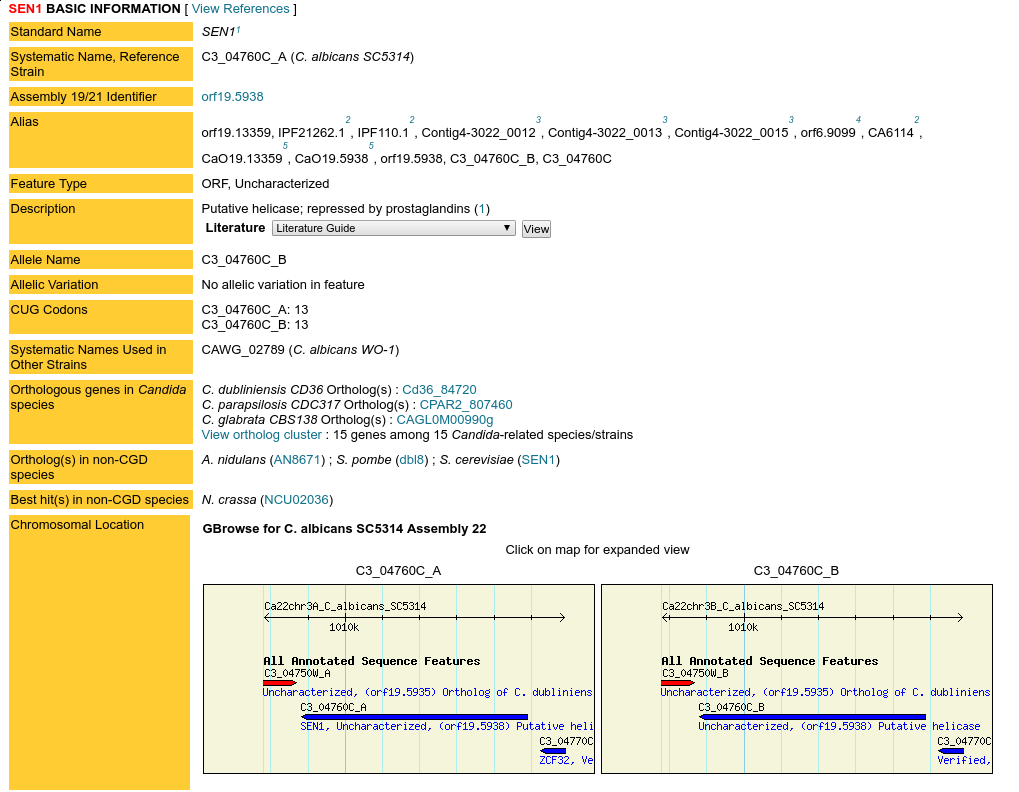
\includegraphics[scale=0.40]{cgd-locus}
\caption{Candida Genome Databases's locus page}
\end{center}
\end{figure}

Next the Yeast Genome\cite{sgd} project's locus page was inspected:

\begin{figure}[H]
\begin{center}
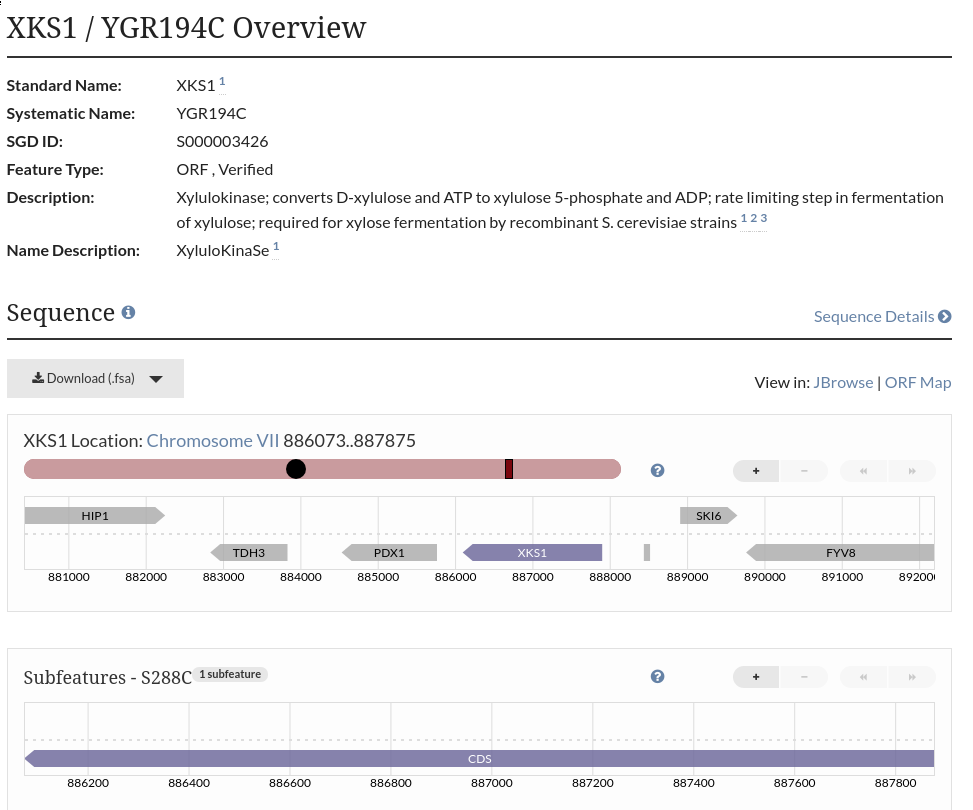
\includegraphics[scale=0.40]{sgd-locus}
\caption{Yeast Genome Project's locus page}
\end{center}
\end{figure}

This page was very nicely formatted and laid out, it clearly had a lot of development, as it had integrations with two genome browsers as well as a large amount of extra information and graphical representations of the genes locations. Replicating this would be ideal, however it is too far out of the scope of this project, as many extra systems would have to be setup to get this data and make it as interactive.

Much like the rest of this project the UI was prototyped along with the understanding of the data at the time. This means that the UI was evolving with the data, and wasn't truly decided upon and polished until the data that was being displayed was known to be correct, and wouldn't change. Unfortunately this didn't happen until quite late in the project. 

\subsubsection{Final design}
The focus for this design was to make it as simple to implement and use as possible, as this isn't a public facing service it doesn't need to be a cutting edge design aimed at grabbing users attention. Instead it just needs to be functional and represent the data clearly. 

There are only two pages on the website, a search view, and a locus page for specific genes. These share the same template, and adapt based on the data provided to them. The tasks for these pages are simply to display the data in the database, and provide a form to query it.

Tooltips were used to display information about each row. As the site is only going to be used by a couple of researchers there wasn't much benefit to creating a help section or a how to guide on how to use the site, as firstly it has been changing a lot during development and secondly it is quicker to just have a direct conversation with them about areas that they might not understand. However if in the future this were to become a public service, I would create an extra information page that lists more background information about the project, the data and how the website is to be used. 

The page was constructed with bootstrap's\cite{bootstrap} grid system, which allows the content to be dynamically repositioned to fit different size displays.

\begin{figure}[H]
\begin{center}
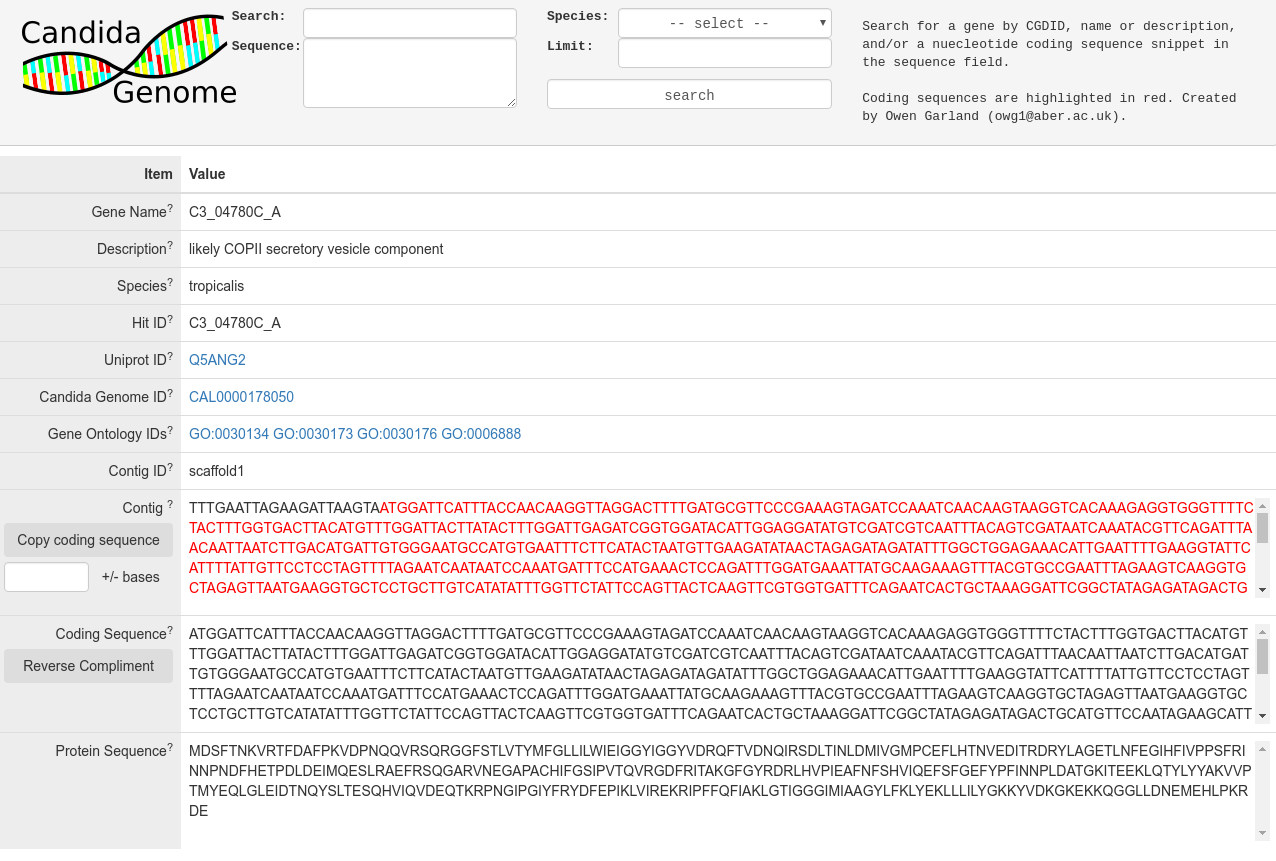
\includegraphics[scale=0.30]{candida-locus}
\caption{The final locus page for the project}
\end{center}
\end{figure}

\begin{figure}[H]
\begin{center}
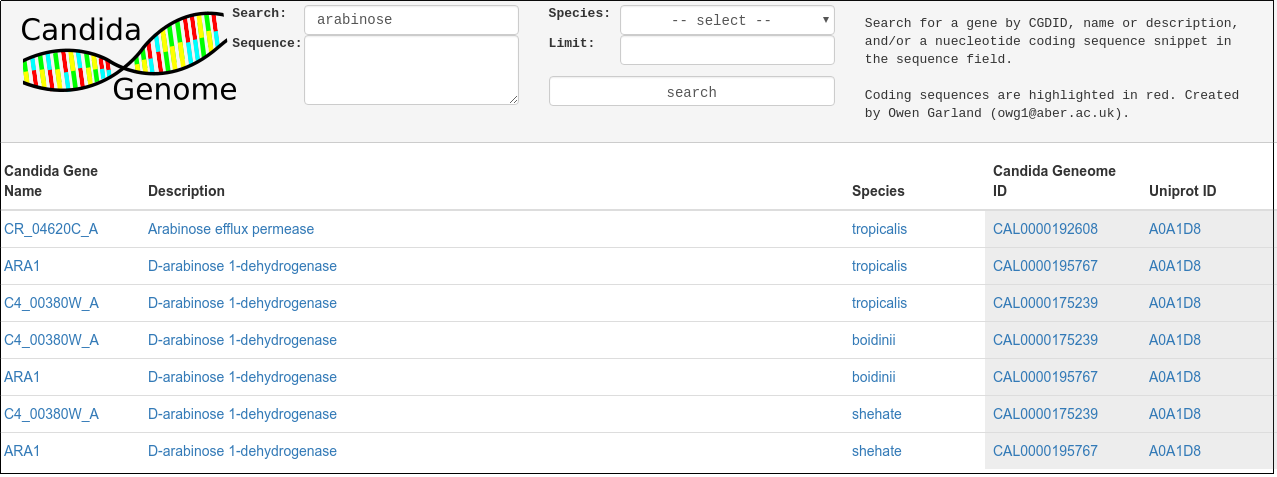
\includegraphics[scale=0.35]{candida-search}
\caption{The final search page for the project}
\end{center}
\end{figure}

\begin{figure}[H]
\begin{center}
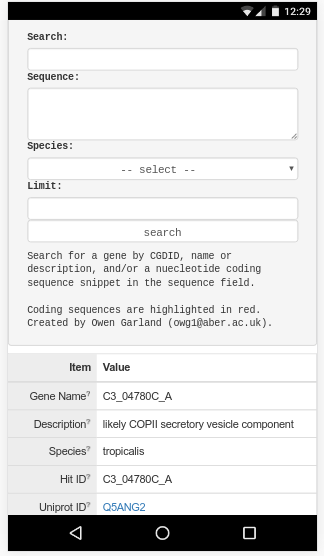
\includegraphics[scale=0.6]{candida-mobile}
\caption{A locus page viewed on a mobile device}
\end{center}
\end{figure}

\begin{figure}[H]
\begin{center}
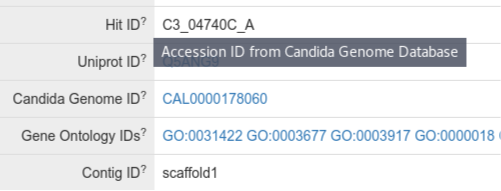
\includegraphics[scale=0.6]{candida-tooltip}
\caption{Tooltip on mouse hover describing what row means}
\end{center}
\end{figure}

\section{Implementation}
During the investigation into the data, many issues were encountered. Mainly due to a lack of understanding of what the data meant, and how it was produced. Initially the plan was to take the raw contigs for each species and use diamond to align them against the NCBI nr database. Then from those results link the data back to the Candida Genome Database via the RefSeq ID's that the NCBI nr database uses. However it was later discovered that there was an annotated set of blast data in the provided data, meaning that this step was no longer necessary.

A prototype was built around this blast data, however it was then realised that the data for \textit{C. boidinii} was not aligned against the NCBI nr database, but rather another unknown data set. This meant that to pursue this line of prototyping I would need to either reproduce the \textit{C. Boidinii} dataset, or reproduce all three with another pipeline, as the results from the alignments weren't consistent. 

The core problem was that it was unknown what tools had been used to produce this data, it appeared that a proprietary tool blast2go\cite{blast2go} had been used to align and annotate the data. However after using a trial copy to try and replicate the results it was evident that this tool had not actually been used to create the alignments with the NCBI nr database. 

Eventually it became clear that the alignment had just been performed with the BLAST tool, on the universities high performance cluster, with an XML format that wasn't known to have existed at the time. This meant that the data could actually be reproduced quite easily with Diamond, using the newly discovered XML output that BLAST offers.

After these revelations, and another meeting with the researchers, we discovered in the original datasets that there were in fact already annotated protein sequence files and coding sequence files.

This meant that the data was already processed and largely annotated already. This meant that it wasn't needed to generate our own data set. There was however one missing piece which was the link back to the Candida Genome Database, something that would be invaluable to the researchers who were already familiar with CGD. 

Because of this, thankfully the weeks of effort spent learning about alignments and annotations weren't wasted, as I was able to produce a new alignment using Diamond. Comparing the coding sequence files, against the proteins found in \textit{C. albicans}, the latter being provided by CGD. This data generated was then able to be used to link the coding sequences found in our data sets to the well documented genes in \textit{C. albicans}. In addition to this the other annotations provided by the original dataset, such as Gene Ontology ID's, are able to be enhanced by using a mapping from the Candida Genome Database to get UniprotKB ID's which offer even more information on the known genes. 

Now each species had, the raw assembled contigs, the coding sequences, the amino acid sequences, the annotated protein information, a link to the Candida Genome Database, and in some cases a link to the UniprotKB database.

The next key piece of information to recover that would be of great use to the researchers was the position of the gene (coding sequence) inside the raw assembled contig. With this information they would be able to easily find the sequence of bases that surround the gene, making wet lab tests a lot easier. 

To do this mock data was produced manually, that contained the correct results, and unit tests made to check if a dummy function was returning the correct results as defined in the mock data. Then an algorithm was developed to find the position of a coding sequence inside a contig. 

The initial algorithm was finding around fifty percent of the genes in the dataset, which was a worry. Thankfully after some discussions with my tutor, it became apparent that the reason for this is that the coding sequences were stored "in one direction", but the alignment results were finding genes that were the reverse compliment of that. This explains why around fifty percent of the genes weren't found. 

Modifying the algorithm to search for the reverse compliment of the coding sequence if it wasn't found "the first way", resulted in every gene being detected. The algorithm, simply found the index of the first twelve bases of the coding sequence in the contig, and the last twelve bases of the coding sequence in the contig. If the start or end couldn't be found it was assumed that the gene was spread across two contigs and the start or end respectively were marked to indicate that the gene was split across two contigs. 

\begin{figure}[H]
\begin{center}
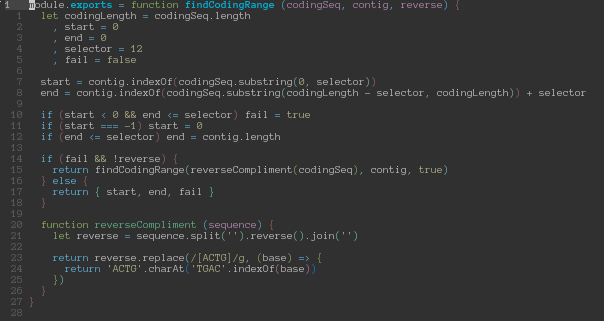
\includegraphics[scale=0.70]{code1}
\caption{Algorithm to find coding sequence inside a contig. \label{overflow}}
\end{center}
\end{figure}

\subsubsection{Search functionality}
Implementation of the search feature underwent several iterations, initially a search based on a regex match was implemented. This meant that each field was searched individually for any subset of the query string. This was very powerful as it would allow substrings to be found for each property of the searched for term. 

An example of this would be if "glucose-6" was searched in the description field, all documents in the database with that string in the description would be returned. This could then be combined with other fields to narrow down the query. 

This implementation was done during the prototyping phase to get a very basic search working for testing purposes, the reason it wasn't going to remain in the application is that a project wide regex search is very inefficient as the search has to be matched against every value int eh entire database for every single query made. Something that would have slowed down the site to unusable levels of performance.

A better solution was to create a generic search field using MongoDB's textSearch\cite{textsearch} feature, that utilises pre-compiled indexes to lookup data in a much more advanced manner. Indexing is quite an intensive task, however for this application where the data is only being read from the service, there is only a need to generate an index once, when the data is being imported to the database, this means the negative impact of an index isn't really in effect, as the import stage is a one time event. 

The fields indexed for the text search are the gene name, protein description, Uniprot ID and Candida Genome ID. Weights are then applied to each field to determine their value when sorting the results of a search. For example a match with a Uniprot ID is weighted higher than a protein description, allowing for results that have a match to a Uniprot ID are sorted higher than those without.  

With this system in place the search was functioning very well, however there was an issue, if a search returned a large amount of documents back, the sort was unable to be ran due to the default MongoDB sort buffer limit. To get around this issue the search function was re-written as an aggregate function. Aggregate\cite{aggregate} in MongoDB allows for a pipeline of steps to be applied to a query, as well as the option to use disk if memory limits are reached. 


% This section should discuss issues you encountered as you tried to implement your experiments. What were the results of running the experiments? What conclusions can you draw from these results? 
% 
% During the work, you might have found that elements of your experiments were unnecessary or overly complex; perhaps third party libraries were available that simplified some of the functions that you intended to implement. If things were easier in some areas, then how did you adapt your project to take account of your findings?
% 
% It is more likely that things were more complex than you first thought. In particular, were there any problems or difficulties that you found during implementation that you had to address? Did such problems simply delay you or were they more significant? 
% 
% If you had multiple experiments to run, it may be sensible to discuss each experiment in separate sections. 

\section{Testing}
Initially it was planned to develop this application in a test driven manner, as it leads to high quality code and stable solutions. 

The difficulty with this approach was that when developing prototypes rapid development is key, as it allows you to try out many different solutions. If a strict TDD pattern was followed during this phase the prototyping would have been drastically slowed as the amount of development work would have doubled. Unfortunately this wasn't a worthy endeavour as time was limited and developing tests for prototype code that may never end up in the final codebase was not going to be feasible.

Another difficulty in testing this project was that the majority of the projects logic is in the seed script that imports the data into the database. Testing this would be difficult because the only way of really checking the validity of what it was producing was to look at what was in the database and to see if that made sense in a biological context. 

Unfortunately it would be beyond the scope of this project to test the biological accuracy of the data that was imported. However I was able to manually verify that the data was correct at several stages, by aligning sequences from this project against other genomic databases such as the Candida Genome Database\cite{cgd} and the Yeast Genome\cite{sgd} project. 

\subsection{Automated Testing}
For the area's of logic that were testable, a TDD design was followed, mainly for the selection of the coding sequence in the contig, as this was the only real area of logic in the project that had it's own custom algorithm to be tested. In addition to this the test suite that was being used for the project also checked the project for code formatting issues with the eslint\cite{eslint} tool. This will cause the tests to fail if potentially dangerous assertions are made in the code. For example if a `==` was used instead of a `===` it will throw and error highlighting the issue to the developer. 

\subsubsection{Unit Tests}
Where possible test driven development was used to produce unit tests, these were mainly written for the logic that detects the coding sequence inside the contig. This is a crucial algorithm as the sites functionality depends on this data being accurate, so it was important that the algorithm be thoroughly tested. To do this several mock database records were created that had all the different possibilities that a gene could be found in, a normal hit, a reverse compliment hit, a missing hit and a hit that was split above and below the contig. 

Tests were then written to compare the result of the finding function against the correct values stored in the mock data. You can see this in the file `find-coding-range.test.js' where the tests are located. The function was then able to be developed ensuring that the data it was returning was correct. 

\subsection{User Interface Testing}
The user interface hasn't had automated tests written for it unfortunately, as there was only one HTML page and only two sets of data that were being returned it didn't feel particularly necessary to write tests to check that the data was coming through correctly. 

That being said the UI has been manually tested on Chrome, Firefox and Internet Explorer to check for any functional issues. None were found, however it was noted that in Internet Explorer there was some font rendering issues, but this isn't a concern as it doesn't impact the functionality of the site. I will be recommending that the site is used on Chrome though, as that it was it was developed on, so is the most thoroughly tested. 

Once the site was at a stage where it could be demonstrated the UI was shown to the researchers and they were asked to provide any feedback that might make the site easier to use for them. This feedback was.... yaydadada .... because of this feedback xyz was done to make it abc for them to use.

\subsection{Stress Testing}
As this site is hosting commercially sensitive data, it won't be publicly accessible, this means that only the researchers who are working on this data will be accessing it. Because of this there isn't a need to perform any stress testing on the service, as the stack is more than capable of handling < 10 users at a time, and isn't vulnerable to public attacks. 

\subsection{Integration Testing}
As listed in the build process section 3.2.4, continuous integration services were used throughout this project, meaning that every time a new build was pushed to github, it had to pass tests on the CI server before being deployed to the production server. This has ensured that any modifications to the code base won't break the core functionality of the production build. 

\subsection{User Testing}
Once the site has been developed to a stage where the users can get a real sense of how it is looking and how it will function, they have been invited to suggest changes that need to be made, in line with the agile practices that this project has been developed with. 

User testing was invaluable as the researchers were able to spot mistakes in the biological data that were invisible to the developer. An instance of this is when they noted that one of the UniprotID's was linking to a gene found in the Flu virus, something that shouldn't be present at all in the yeast genome. After investigating it was found that some of the UniprotID's has been truncated which caused this anomaly. Writing tests for these kinds of checks would have been nigh on impossible, thankfully user tests were able to pick up these kinds of issues. 

% Detailed descriptions of every test case are definitely not what is required here. What is important is to show that you adopted a sensible strategy that was, in principle, capable of testing the system adequately even if you did not have the time to test the system fully.

% Provide information in the body of your report and the appendix to explain the testing that has been performed. How does this testing address the requirements and design for the project?

% How comprehensive is the testing within the constraints of the project?  Are you testing the normal working behaviour? Are you testing the exceptional behaviour, e.g. error conditions? Are you testing security issues if they are relevant for your project? 

% Have you tested your system on ``real users''? For example, if your system is supposed to solve a problem for a business, then it would be appropriate to present your approach to involve the users in the testing process and to record the results that you obtained. Depending on the level of detail, it is likely that you would put any detailed results in an appendix.

% The following sections indicate some areas you might include. Other sections may be more appropriate to your project. 
